\documentclass[%
12pt, %
final, % 
oneside, % 
onecolumn, %  
centertags]{article} % относится к классу article и размер шрифта 12 пунктовб, {article: статья, report: отчеты и диссертации, book: книга, letter: письмо}

% \usepackage{fontspec}
 
% \setmainfont{Times New Roman}

% \documentclass[a4paper, 12pt]{report}

\topmargin= -30pt % насколько сверху будет страница
\textheight= 650pt


\usepackage[utf8]{inputenc} % задает кодировку, utf-8 кодировка, включающая в себя знаки почти всех языков мира
\usepackage[english]{babel} % подключает необходимые языки, основным языком является английский

\selectlanguage{english} % настройки будут на английском, но писать будет на русском

\usepackage{euscript}
\usepackage{supertabular}

\renewcommand{\baselinestretch}{1.0} 

\usepackage[colorlinks=true,linkcolor=blue,unicode=true,urlcolor = blue]{hyperref} %hypered
\usepackage[pdftex]{graphicx} % для графики

\usepackage{amsthm, amssymb, amsmath, amsfonts} % математический пакет, математические шрифты
\usepackage{textcomp}
\usepackage[noend]{algorithmic}
\usepackage[ruled]{algorithm}
\usepackage{lipsum}
\usepackage{indentfirst}
\usepackage{babel}
\usepackage{pgfplots}
\usepackage{setspace}
\usepackage{xcolor}
\usepackage{hyperref}
\usepackage{subfigure}

\setcounter{secnumdepth}{5}
\setcounter{tocdepth}{5}
\newcommand\simpleparagraph[1]{%
  \stepcounter{paragraph}\paragraph*{\theparagraph\quad{}#1}}
\usepackage{listings}
% \usepackage{xcolor}
%\usepackage{minted}

\lstset { %
     language=C++,
     backgroundcolor=\color{black!5}, % set backgroundcolor
     basicstyle=\footnotesize,% basic font setting
}


\linespread{1.0} 
\setlength{\parindent}{2.4em}
\setlength{\parskip}{0.1em}

\pgfplotsset{compat=1.9}
\pgfplotsset{model/.style = {blue, samples = 100}} 
\pgfplotsset{experiment/.style = {red}}

\theoremstyle{plain}
\binoppenalty=10000

\newtheorem{theorem}{Theorem}[section] % theorem

\theoremstyle{definition}
% \newtheorem{definition}{Определение}[subsection]
\newtheorem{definition}{Definition}[subsection]

\theoremstyle{remark}
% \newtheorem{remark}{Замечание}[section]

% \newtheorem{corollary}{Следствие}

% \newtheorem{proposition}{Proposition}

% \newtheorem{example}{Пример}

% \newtheorem{lemma}{Лемма}[section]

\renewcommand*{\proofname}{Proof}

\graphicspath{ {./images/} }


% \usepackage{amsmath,amsfonts,amssymb, setspace}  % Разнообразные математические команды и значки
% \usepackage{indentfirst}     % Отступ в первом абзаце

% \pagestyle{empty}
\usepackage[left=2.5cm, right=1.5cm, top=2.5cm, bottom=2.5cm]{geometry}
\usepackage[medium]{titlesec}
\usepackage{graphicx}
% \graphicspath{ {./images/} }

\begin{document}

	\begin{titlepage} 
		\begin{center}
		\textbf{}\\[2.0cm]
		\LARGE FEDERAL STATE AUTONOMOUS EDUCATIONAL INSTITUTION OF HIGHER EDUCATION \\[0.5cm]
		\Large ITMO UNIVERSITY \\[3cm]
		\LARGE Report\\
		\Large MPI. Assignments $8$ \\
		\Large Parallel algorithms for the analysis and synthesis of data \\[4cm]


		\begin{flushright}
		Performed by\\
		Aleksandr Shirokov\\
		J4133c\\
		Accepted by\\
		Petr Andriushchenko

		Deadline: 20.12.21
		\end{flushright}

		\vfill 

		{\Large {St. Petersburg}} \par
		{\Large {2021}}
		\end{center} 
	\end{titlepage}

\tableofcontents
\newpage


\section{Assignments}

\subsection{Assignment 8. MPI.  Bandwidth measurement.}

\subsubsection{Formulation of the problem}

\begin{enumerate}
	\item Write an MPI program in which two processes exchange messages
	\item Measure the time 
per exchange iteration
	\item Determine the dependence of the exchange time on the 
message length.
	\item Determine the latency and maximum achievable bandwidth of the 
communication network.
	\item Print the message length in bytes and the throughput in 
MB/s to the console.
	\item Change the length of the message in a loop starting from $1$ element and increase to $1,000,000$ elements, increasing by $10$ times at each iteration.
\end{enumerate}

\subsubsection{Bandwidth measurement technique}

The following technique is used to measure point-to-point bandwidth. Process $0$ sends a message of length $L$ bytes to process $1$.

$$L = \operatorname{number \ of \ elements} \cdot \operatorname{length \ in \ bytes \ of \  data \ type}$$
$$L = 100 \cdot \operatorname{sizeof}(int)$$

Process $1$, having received a message from process $0$, sends it a reply message ot the same length. Blocking MPI calls are used (\textsc{MPI\_Send}, \textsc{MPI\_Recv}). These actions are repeated $N=10$ times in order to minimize the error due to averaging. Process $0$ measures the time $T$ taken for all these exchanges.

The bandwidth $R$ is determined by formula:

$$R = \frac{2NL}{T}$$

\subsubsection{Latency measurement technique}

Latency is measured as the time it takes to transmit a signal or message of zero 
length. At the same time, to reduce the influence of the error and low resolution of 
the system timer, it is important to repeat the operation of sending a signal and 
receiving a response a large number of times.

Thus, if the time for $N$ iterations of sending zero-length messages back and forth was $T$ sec., Then the latency is 
measured as:

$$s = \frac{T}{2N}$$

\subsubsection{Example of launch parameters and output. Detailed description of solution}

Code for \textbf{assignment 6} is \href{https:\//github.com/aptmess/parallel_algorithms/blob/master/HT/hw_mpi/Assignment8.c}{here}.

Compilation example: \textsc{mpic++ -o ./cpf/8.o Assignment8.c}

Launch example: \textsc{mpirun --oversubscribe -np 2 ./cpf/8.o}

\begin{center}
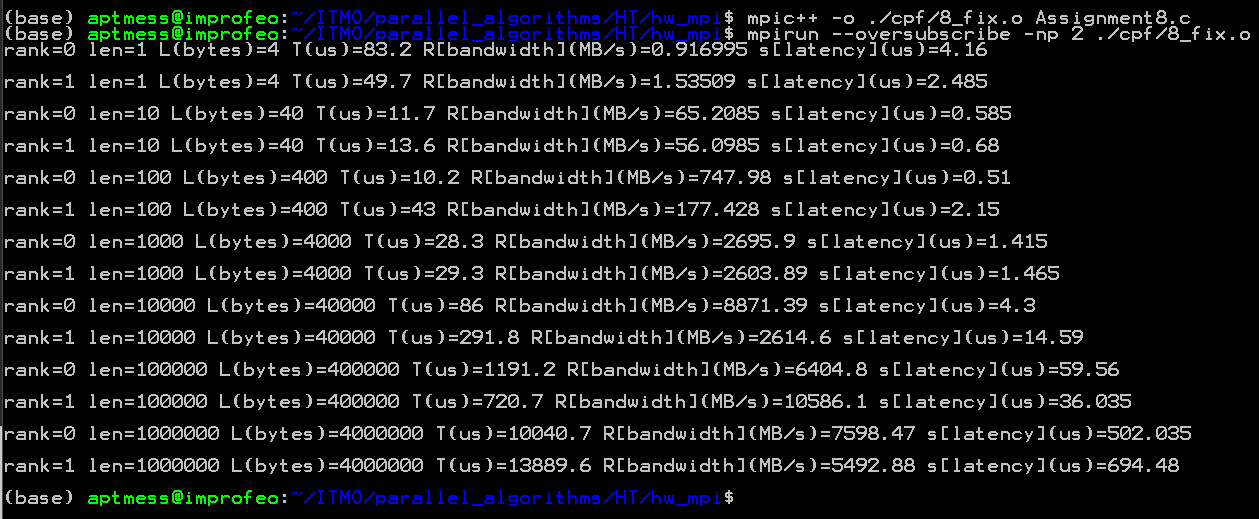
\includegraphics[scale=0.5]{8.3.png}
\end{center}
% \begin{center}
% 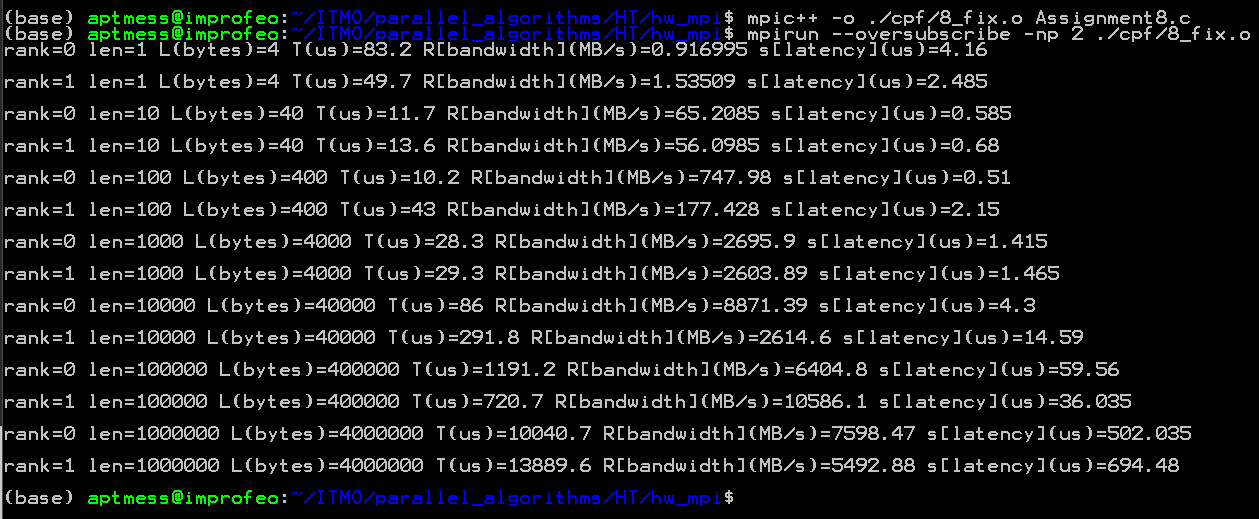
\includegraphics[scale=0.75]{8.3.png}
% \end{center}

Let's move to the the code and explain how it works.

\begin{figure}[h!]
\centering
\subfigure{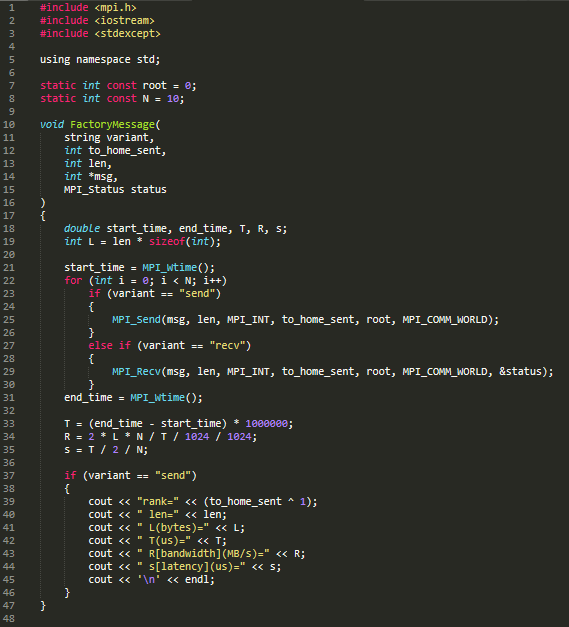
\includegraphics[width=0.47\textwidth]{8.1.code.png}} 
\subfigure{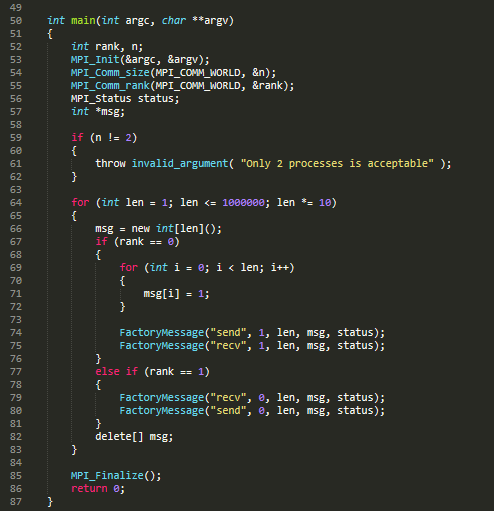
\includegraphics[width=0.5\textwidth]{8.2.code.png}} 

Assignment8 code
\end{figure}

In the code there are on function \textsc{FactoryMessage}, that start \textsc{MPI\_Send} or \textsc{MPI\_Recv} function depends on input parameter \textit{variant}, after that there are a computation of metrics such as average time in seconds, latency and bandwidth by formulas in previous subsections and printing the result. In main function process $0$ send array of different length on each iteration of for cycle to process $1$, process $1$ then recieves it and send to process $0$ and it is continue for cycle $\operatorname{len}=[1..1000000]$ by increasing it $10$ times in each iteration. 

We can also check if results are more or less correct - I tried to compare latency from \href{https:\//www.intel.com/content/www/us/en/high-performance-computing-fabrics/omni-path-architecture-performance-overview.html}{intel} comparison and it is more or less the same as in our experiement!

\begin{figure}[h!]
\centering
\subfigure{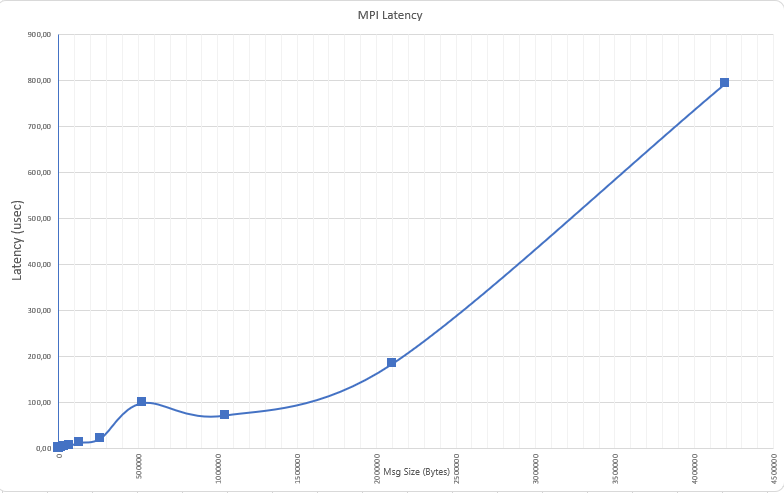
\includegraphics[width=0.6\textwidth]{8.1.lat.png}} 
\subfigure{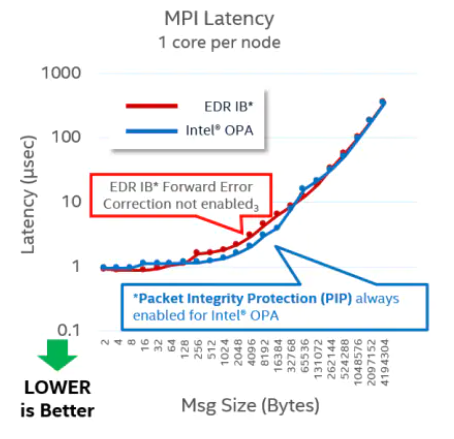
\includegraphics[width=0.4\textwidth]{8.latency.png}} 

Experiement by Intel of MPI latency and our - looks similar
\end{figure}

We have explained the code in assignment 8 and compare the results.

\subsection{Appendix}

The link to the sourse code which is placed on my \href{https://github.com/aptmess/parallel_algorithms}{github}.


\end{document}